\section{Algoritme til detektering af cykling}\label{sec:algocykel}
\textit{Dette afsnit omhandler design, implementering og test af algoritmen til detektering af cykling. Først designes algoritmen til det specifikke formål, hvorefter den kan implementeres. Afslutningsvist bliver algoritmen testet i forhold til opstillede krav i \secref{krav_algoritme}.} 

For at kunne detektere cykling og adskille dette signal fra gang og løb benyttes et gyroskop, som er beskrevet i \secref{sec_design_LSM9DS1}. Signalet herfra skal databehandles, således det opfattes anderledes af GUIen i det samlede system og derved opfanges som aktiviteten cykling. 

\subsection{Design}\label{design_cykling}
Data fra gyroskopets z-akse skal signalbehandles, førend en algoritme kan detektere cykling og adskille denne fra gang og løb. Første trin i denne signalbehandling er at udføre en Fast Fourier Transform (FFT) over fire sekunders sampling. Dette medfører, at signalets frekvenser og deres tilhørende magnituder kommer til udtryk. I andet trin findes frekvensværdien for den maksimale peak. Amplituden herfra bliver summeret i det tredje trin sammen med amplituderne for $\pm$1 Hz af den pågældende frekvens med maks peak. Derved fås en amplitudeværdi for maks peak værdien summeret med de to omkringliggende amplitudeværdier. Derudover summeres amplitudeværdierne for FFTen fra 1 til 20 Hz i det tredje trin, som herefter vil blive betegnet som hele FFTen. Resultatet heraf består i en amplitudeværdi for den maksimale peak med omkringliggende værdier, samt en amplitude værdi for hele FFTen. Resultaterne af disse to summeringer benyttes til fjerde og sidste trin, som omregner hvor stor en procentdel den første summering med det højeste peak udgør i forhold til den samlede FFT. Summeringen over den maksimale peak med omkringliggende værdier vil typisk udgøre en stor procentdel af den samlede summering. Resultatet af at summeringen udgør en stor procentdel af den samlede energi, er at cykling afspejles som et sinussignal, hvoraf energien befinder sig omkring få frekvenser. Aktiviteterne gang og løb har ikke samme karakteristiske påvirkning af gyroskopet.
\begin{figure}[H]
	\centering
	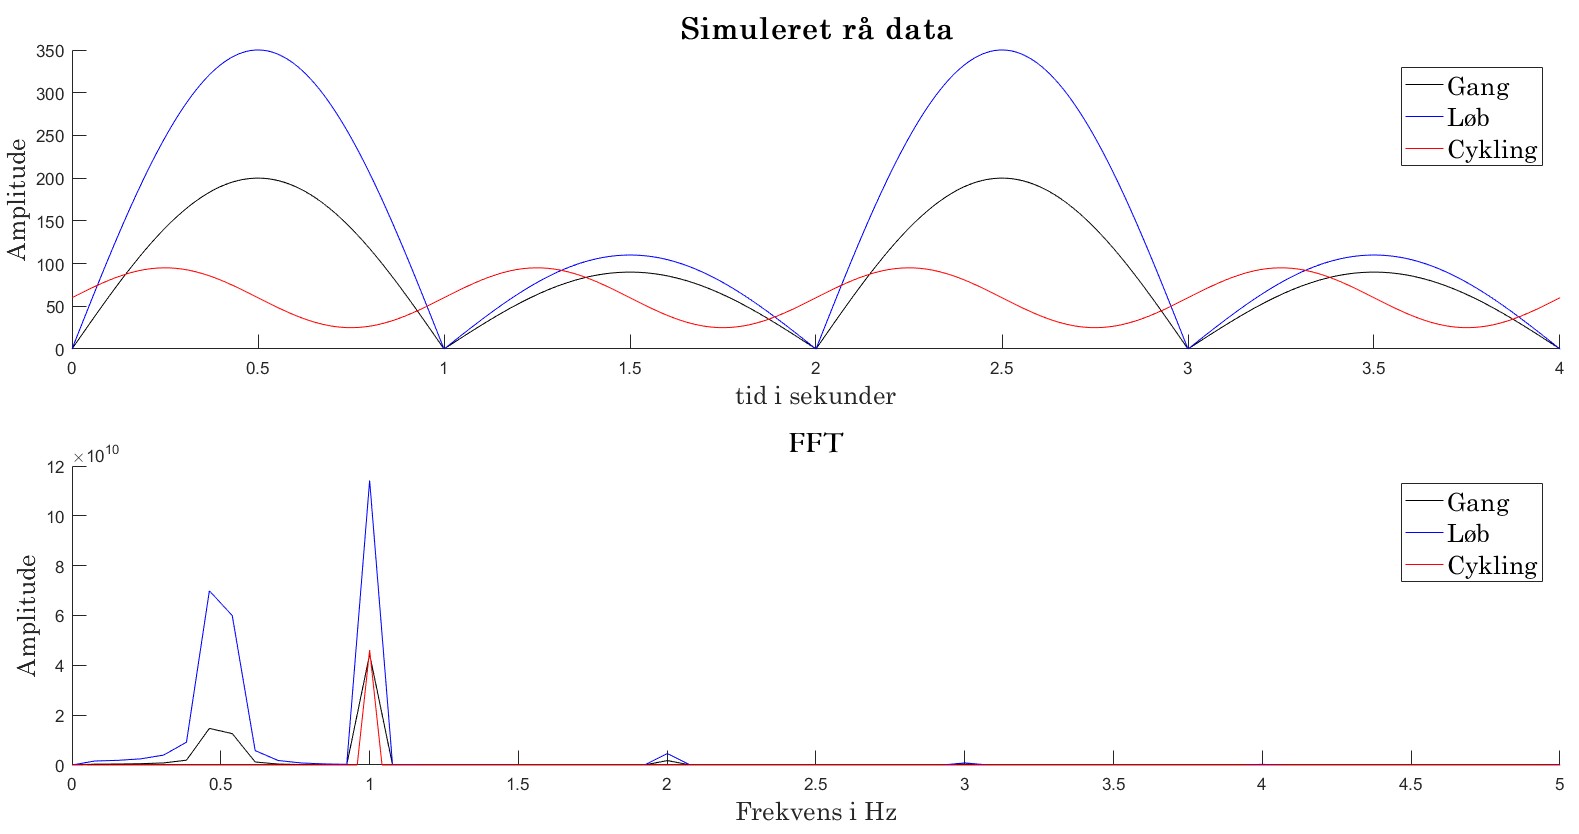
\includegraphics[scale=0.8]{figures/cDesign/gyro_behandling.png}
	\caption{Figuren viser rå data for gang, løb og cykling for et 5 sekunders interval opsamlet på gyroskopets z-akse på øverste graf, samt signalbehandling af dataet fra 0 til 20~Hz på nederste graf.}
	\label{fig:gyro_behandling}
\end{figure}\vspace{-0.5cm}
Data fra pilotforsøget er behandlet med ovenstående signalbehandling. Dette er gjort med henblik på fastsættelse af en tærskelværdi som adskiller cykling fra gang og løb. På den øverste graf på \figref{fig:gyro_behandling} ses de rå signaler fra gyroskopet fra gang, løb og cykling. Som det tydelig ses afspejles cykling tilnærmelsesvis som en sinus, hvorfor dennes energi er centreret omkring få frekvenser. Resultatet af den omtalte signalbehandling ses på den nederste graf, hvoraf gang, løb og cykling er blevet behandlet med en FFT. Hertil ses det også at energien for gang og løb ikke centrerer sig omkring en enkelt frekvens, men om forskellige frekvenser, hvoraf denne spredning af energi kan benyttes til signalgenkendelse og adskillelse af aktiviteterne. 

Efter ovenstående signalbehandlingen implementeres signalgenkendelsen som består af, først at finde den maksimale magnitude og den tilhørende frekvens, resultatet heraf er aktivitetens dominerende frekvens. Herefter summeres værdierne for den maksimale magnitude, ved at summere intervallet $\pm$1~Hz omkring frekvens heraf. Hertil summeres også værdierne for FFTen fra 1 til 20~Hz. Afslutningsvist bestemmes hvor stor en procentdel summeringen for den maksimale magnitude udgør af summeringen for 1 til 20~Hz.\\ 

\begin{table}[H]
	\centering
		\begin{tabular}{cccc}
			\hline
			\rowcolor[HTML]{C0C0C0} 
			Forsøgsperson & Procentdel af totalen for gang & Procentdel af totalen for løb & Procentdel af totalen for cykling \\ \hline
			F1 & 41,0\% & 38,6\% & 85,5\% \\ \hline	
			F2 & 48,5\% & 51,5\% & 91,9\% \\ \hline	
			F3 & 35,9\% & 42,8\% & 85,0\% \\ \hline
			F4 & 38,7\% & 60,6\% & 91,6\% \\ \hline
		\end{tabular}
	\caption{I tabellen ses hvor stor en procentdel summeringen vedrørende den maksimale magnitude udgør af hele FFTen. Dette er gjort for både gang, løb og cykling, med henblik på bestemmelse af en tærskelværdi.}
	\label{tab:individuel_procent}
\end{table}\vspace{-0.5cm}
Mængden af energi ved den maksimale magnitude er markant større for cykling i forhold til gang og løb, hvilket er illustreret i \tabref{tab:individuel_procent}. Dette resulterede i, at 84,5\% til 91,9\% af energien lå $\pm$1 Hz omkring den fundne frekvens med den største amplitude. Hvorledes acceleration eller andre hastigheder ved cykling har påvirkning på denne procentfordeling diskuteres i \secref{sec:diskussion}. Procentfordelingen blev ligeledes behandlet for gang og løb for at sikre, at disse ikke havde samme spredning i frekvensområdet, hvormed en mulig tærskelværdi til detektering af cykling kan fastsættes. Resultatet heraf medførte at ved gang befandt energien omkring den fundne frekvens sig mellem 35,9\% til 48,5\% og ved løb befandt energien omkring den fundne frekvens sig mellem 42,8\% til 60,5\%. Denne forskel benyttes til at adskille cykling fra gang og løb, ved at implementere et tærskelværdi på 70\%. Summeringen af magnituden omrking den største magnitude skal dermed udgøre 70\% for at blive klassificeret som cykling. 
\begin{figure}[H]
	\centering
	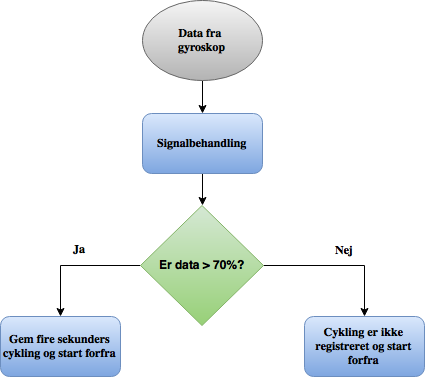
\includegraphics[scale=0.6]{figures/cDesign/algoritme_cykling.png}
	\caption{På figuren ses et flowchart som gennemgår algoritmen vedrørende detektering af cykling.}
	\label{fig:algoritme_cykling}
\end{figure}
Ovenstående figur repræsenterer algoritmen for detektering af cykling. Hvis cykling detekteres, starter en time count, som stopper når cykling ikke længere detekteres. Når timeren stopper, videresendes timerens værdi som repræsenterer tiden hvormed cykling har været detekteret. Hvis cykling ikke detekteres, signalbehandles ny data fra gyroskopet, for at tjekke hvorvidt cykling detekteres.
%Data fra gyroskopets z-akse skal signalbehandles, førend en algoritme kan detektere og adskille aktiviteterne. Første step i denne signalbehandling er at udføre en Fast Fourier Transform (FFT) over to sekunders sampling. Dette medfører at signalets magnitude og dets tilhørende frekvenser kommer til udtryk, hvoraf andet step indledes. Dette step finder den maksimale magnitude med tilhørende frekvens. Tredje step består af to integraler, første integrale integrer FFT'en fra den frekvens hvor den største magnitude befandt sig $\pm 1$Hz. Andet integrale integrer FFT'en fra 1 til 20 Hz. Disse integraler indleder fjerde og sidste step, som omregner hvor stor en procentdel første integrale udgør af signalets totale energi. \\
%Resultatet af ovenstående signalbehandling medfører at der opstilles et udtryk for signalets spredning af energi. Det gør sig gældende at cykling har en spredning af energi fordelt nært frekvensen med den største amplitude. Data fra gyroskopets z-akse vedrørende cykling blev for alle forsøgspersoner, behandlet med ovenstående metode. Dette resulterede i at 84,2\% til 88,4\% af energien lå $\pm 1$Hz omkring den fundne frekvens. Følgende blev ligeledes behandlet for gang og løb, for at sikre disse ikke havde samme spredning i frekvensområdet, hvormed en mulig tærskelværdi til detektering af cykling, kan fastsættes.  Dette resulterede i at ved gang befandt energien omkring den fundne frekvens sig mellem 47,2\% til 55,4\% og ved løb befandt energien omkring den fundne frekvens sig mellem 42\% til 50,6\%. \\
%Resultatet af at energien omkring den fundne frekvens med den største amplitude er $\approx$30\% større ved cykling end ved gang og løb, fastsættes tærskelværdien til 70\%. For at detektere cykling skal outputtet fra databehandlingen være større end 70\%.

\subsection{Implementering}
Implementeringen af algoritmen for detektering af cykling tager udgangspunkt i data fra pilotforsøget og de designmæssige aspekter, som er beskrevet i \secref{design_cykling}. Algoritmen er designet og implementeret, som det ses på \figref{fig:basic_cykling}.
\begin{figure}[H]
	\centering
	\includegraphics[scale=0.4]{figures/cDesign/Algoritme_cykling_basic.png}
	\caption{På figuren ses den kode for algoritmen til detektering cykling beskrevet med pesudokode. Den røde markerede kasse vil blive forklaret yderligere en kommende figur.}
	\label{fig:basic_cykling}
\end{figure}
Algoritmen henter low-, og high byte fra ICens gyroskop outputdata, hvorefter hver enkelt sample videresendes til MATLAB, som gemmer 4 sekunders data i et arrary og påbegynder signalbehandlingen. Resultatet af signalbehandlingen medfører en procentvis værdi for det modtagne data. Denne værdi undersøges for at være over eller under tærskelværdien. Hvis resultatet er over 70\% summeres fire sekunder til den totale varighed for cykling, hvis ikke startes algoritmen forfra.
\begin{figure}[H]
	\centering
	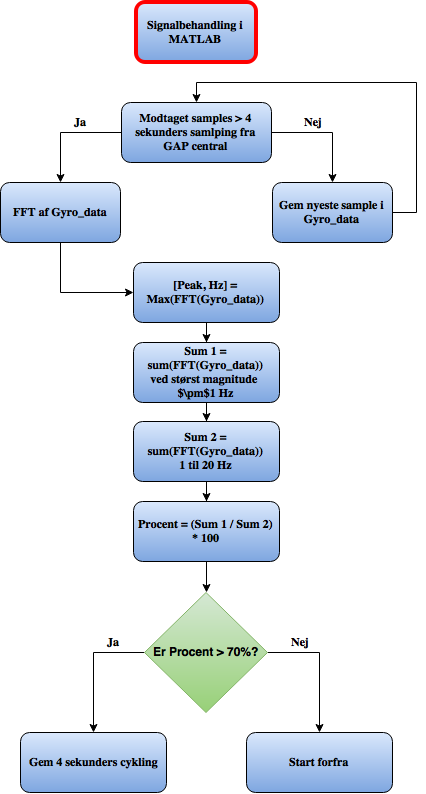
\includegraphics[scale=0.4]{figures/cDesign/algoritme_matlab_cykling.png}
	\caption{På figuren ses den kode for algoritmens signalbehandling i MATLAB.}
	\label{fig:matlab_cykling}
\end{figure} 
Når MATLAB har modtaget fire sekunders sampling påbegyndes signalbehandlingen af dataet ved brug at formlerne i \figref{fig:matlab_cykling}. Hvis cykling bliver detekteret bliver en varighed på fire sekunder videresendt til udført cykling i GUI. 


\subsection{Test}
%Algoritmen til detektion af cykling skal testes for følgende krav fra \secref{krav_algoritme}:
%\begin{itemize}
%	\item Behandle data fra gyroskopet således, at frekvensindholdet fra signalet fremstår.
%	\item Være i stand til at detektere henholdsvis gang, løb og cykling ved hjælp af tærskelværdier for peakværdien eller procentfordeling af frekvensindhold. Der accepteres ikke, at systemet ikke kan detektere og adskille de tre aktivitetsformer.
%\end{itemize}

Algoritmens funktioner testes individuelt og samlet ligeledes som med algoritmen for gang og løb. Dette gøres for at be- eller afkræfte om algoritmen lever op til de opstillede krav i \secref{krav_algoritme}, som lyder at algoritmen skal:
\begin{itemize}
	\item Indlede med databehandling således, %hælnedslaget fra accelerometrets optagede data fremstår som en tydelig peak, og 
	gyroskopets data for cykling fremstår som en tydelig sinus. %Der accepteres ikke, hvis signalet ikke kommer til at fremstå som en tydelig peak eller sinus.
	\item Være i stand til at detektere henholdsvis gang, løb og cykling ved hjælp af eksempelvis tærskelværdier for peakværdien. Der accepteres ikke, at systemet ikke kan detektere og adskille de tre aktivitetsformer.
\end{itemize}

Måden hvorpå dette testes er ved at indsende et simuleret signal, hvis funktion er at agerer som gang, løb eller cykling. De simulerede signaler for gang og løb er genereret som kombinationer af absolutte sinussignaler med varierende amplitude, mens signalet for cykling er en sinus forskudt på y-aksen, således at disse tilnærmelsesvis ligner signalerne fra pilotforsøget.

Det første som testes, er algoritmes 4 sekunders tæller... \fxnote{skrives færdig når testen virker.}

Den anden test som laves, omhandler hvorledes FFTen stemmer overens med forventningerne hertil. Da sinussignalet som repræsenterer cykling har en frekvens på 1~Hz, forventes det at plottet for FFTen illustrerer at dette signal danner en peak omkring 1~Hz. Ved gang og løb, som begge er kombinationer af absolutte sinussignaler med varierende amplituder, forventes det at FFTen for disse centrerer sig omkring flere forskellige frekvenser. Resultatet af denne test ses illustreret på \figref{fig:sim_gryo}, hvor de simulerede rå signaler ses på øverste graf, mens FFTen for signalerne ses på nederste graf.

\begin{figure}[H]
	\centering
	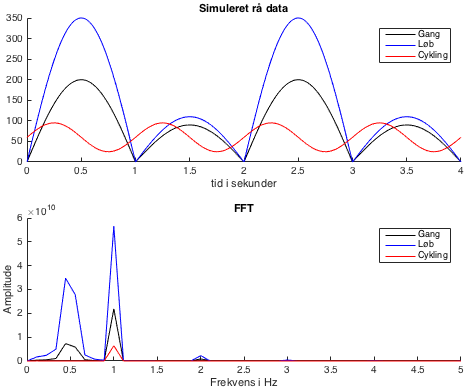
\includegraphics[width=.9\textwidth]{figures/cDesign/sim_gyro.png}
	\caption{På figurens øverste graf ses de simulerede rå signaler for gang, løb og cykling, hvorefter den nederste graf illustrer signalerne efter de er blevet databehandlet.}
	\label{fig:sim_gyro}
\end{figure}

Som forventet ses det på \figref{fig:sim_gyro}, at FFTen for cyklingssignalet centreres omkring 1~Hz, mens signalerne for gang og løb centreres omkring henholdsvis 0,5~Hz, 1~Hz og 2~Hz.\\ 
Da det er forskelligt om de tre signaler centrerer sig omkring én eller flere frekvenser forventes det, at spredningen af signalets energi varierer for de tre aktiviteter, hvilket den tredje test vil undersøge. Heraf forventes det at spredningen af energien ved cykling er markant mindre end spredningen af energi ved gang og løb. Som beskrevet i \secref{design_cykling} forventes minimum 70\% af energien ved cykling, at være indenfor $\pm$1~Hz omkring den maksimale peak af FFTen, hvorimod det ved gang og cykling forventes at være markant mindre. 

\begin{table}[H]
	\centering
	\begin{tabular}{cccc}
		\hline
		\rowcolor[HTML]{C0C0C0} 
		Procent for gang & Procent for løb & Procent for cykling \\ \hline
		56,85\% & 42,46\% & 99,28\% \\ \hline	
	\end{tabular}
	\caption{I tabellen ses hvor mange procent den maksimale frekvensmagnitude udgør af 1-20~Hz ved simuleringerne for gang, løb og cykling.}
	\label{tab:sim_procent}
\end{table}\vspace{-0.5cm}

Som det fremgår af \tabref{tab:sim_procent} udgør energien i den maksimale frekvensamplitude markant mere af den samlede energi ved cykling end ved gang og løb. Det bekræftes derfor at cykling bør kunne registreres ved 70\% af signalet, da det i simuleringen udgør 99,28\%, mens gang og løb maksimalt udgør 56,85\%. 

Afslutningsvist testes det om en tærskelværdi på 70\% vil kunne detektere og gemme de 4 sekunders cykling som er samplet, mens den ikke registrerer gang eller løb. Det testes ligeledes om algoritmen kan detektere cykling i mere end 4 sekunder, ved at der returneres antal gange der er registreret 4 sekunders cykling samt en samlet tidsvariabel.\fxnote{skriv dette færdigt når det virker i matlab} 

